\section{Certified-correction risk control}
\label{sec:method}

\subsection{The policy family}

Fix a gate value $g$ and a descending grid of acceptance thresholds $t_1>\dots>t_M$ on the
channel-1 score. Policy $\pi_j$ acts as
\begin{equation}
\pi_j(x)=
\begin{cases}
\textsc{accept}\ \hat a(x), & s(x)\ge t_j,\\
\textsc{repair with}\ b(x), & s(x)<t_j\ \text{and}\ m(x)\ge g,\\
\textsc{abstain}, & \text{otherwise.}
\end{cases}
\label{eq:policy}
\end{equation}
Figure~\ref{fig:method} shows the induced partition of the $(s,m)$ plane. The emitted set of $\pi_j$
is the accepted set together with the repaired set, and an emitted error is a wrong accepted answer
or a wrong channel-2 answer: with $A_j=\{s\ge t_j\}$ and $R_j=\{s<t_j,\ m\ge g\}$,
\begin{equation}
W_j=\ind{X\in A_j}(1-Y)+\ind{X\in R_j}(1-Y^{(2)}).
\label{eq:err}
\end{equation}
Because $g$ does not depend on $j$, the emitted set $A_j\cup\{m\ge g\}$ grows as $t_j$ falls.
Filtering is the case $g=\infty$.

\begin{figure}[t]
\centering
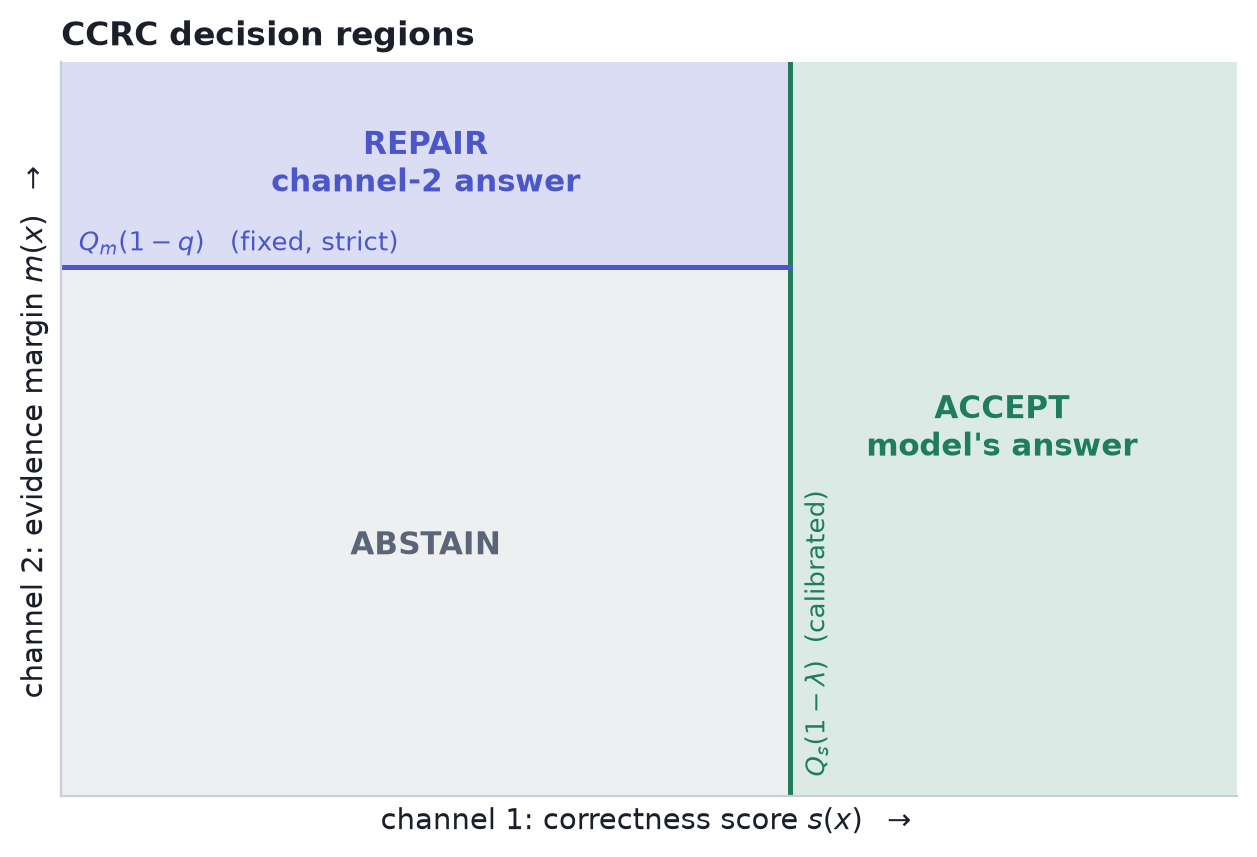
\includegraphics[width=0.55\textwidth]{fig_method.png}
\caption{The $(s,m)$ plane under policy \eqref{eq:policy}. The acceptance threshold moves along the
sequence; the repair gate is fixed, so the accepted region grows while the repair region shrinks.}
\label{fig:method}
\end{figure}

\subsection{How thresholds and gate are fixed}
\label{sec:fixing}

Both are values, and both are computed from the fit fold, which is disjoint from the calibration
fold and from the test fold.
\begin{itemize}
\item \emph{Score grid.} The channel-1 model is fitted on the fit fold. Its out-of-fold scores on
  that fold (image-grouped five-fold cross-fitting inside the fit fold) define the grid
  $t_j=Q_{1-\lambda_j}$ of their empirical distribution, with $\lambda_1<\dots<\lambda_{40}=1$
  equally spaced. Using out-of-fold scores keeps the quantile-to-value map faithful to
  out-of-sample behaviour; an in-sample fit is mildly overconfident on its own data.
\item \emph{Start.} The first hypothesis is where $c\,k_{\mathrm{start}}(e_0)$ items are expected
  to be emitted, $\lambda_1=\min\{0.9,\max\{0.05,\,c\,k_{\mathrm{start}}(e_0)/n_{\mathrm{cal}}\}\}$,
  with $k_{\mathrm{start}}(e_0)=\min\{k:U(e_0,k;\delta)\le\alpha\}$ the smallest emitted count at
  which $e_0$ observed errors still certify the target (Lemma~\ref{lem:kstart}). The default is
  $e_0=1$, $c=1.5$: start where one error can be tolerated, with half as much again as headroom for
  fold-to-fold variation in $K$. The start is computed from $\alpha$, $\delta$ and $n_{\mathrm{cal}}$
  alone, before any label is read; \S\ref{sec:start} ablates it.
\item \emph{Repair gate.} $g=Q_{1-q}(m)$ over grounded fit-fold items. Three ways of fixing
  $q$ keep the guarantee: (a) \emph{external}: $q$ is chosen once on a different benchmark by
  running the same procedure there and keeping the candidate (filtering, or $q\in\{0.05,0.10,0.25,0.50\}$)
  that certifies the most coverage; (b) \emph{fit-fold}: the same choice is made inside each split on the fit
  fold alone; (c) \emph{union}: three gates $\{0.05,0.10,0.25\}$ are each certified at $\delta/3$ and
  the certified policy with the largest calibration coverage is emitted.
\end{itemize}

\subsection{Validity}
\label{sec:validity}

\begin{theorem}[CCRC validity]
\label{thm:validity}
Under Assumptions~\ref{ass:iid} and~\ref{ass:family}, let $\hat\jmath$ be the last index passed by the
fixed-sequence test that proceeds through $j=1,2,\dots$ while $U(V_j,K_j;\delta)\le\alpha$ on the
calibration sample and stops at the first failure ($\hat\jmath=0$ if the first test fails, in which
case nothing is emitted). Then
\[
\Pr\bigl[\Risk(\pi_{\hat\jmath})\le\alpha\bigr]\ \ge\ 1-\delta,
\]
where the probability is over the calibration sample, conditional on the fit data.
\end{theorem}

\begin{proof}
Condition on the fit data, so the policies are fixed. For policy $j$ let $K_j=\sum_i\emit_j(X_i)$ and
$V_j=\sum_iW_j(Z_i)$, and consider $H_j:\Risk(\pi_j)>\alpha$. Emission is a function of $X$ alone.
By Assumption~\ref{ass:iid} the units are independent, so conditional on the set of emitted units
(equivalently, on the emission pattern), the emitted units are i.i.d.\ draws from $P(\cdot\mid\emit_j=1)$
and each has error indicator $W_j\sim\mathrm{Bernoulli}(\Risk(\pi_j))$, independently across units.
Hence $V_j\mid\{K_j=k\}\sim\mathrm{Bin}(k,\Risk(\pi_j))$, and by construction of the
Clopper--Pearson bound, $\Pr[U(V_j,K_j;\delta)\le\alpha\mid K_j=k]\le\delta$ whenever
$\Risk(\pi_j)>\alpha$ and $k\ge1$; for $k=0$ the bound is $1>\alpha$. So $\phi_j=\ind{U\le\alpha}$ is a
level-$\delta$ test of $H_j$.

Let $j_0=\min\{j:H_j\text{ is true}\}$, if it exists. The sequence reaches an index $\ge j_0$ only if $H_{j_0}$
is rejected, an event of probability at most $\delta$. On the complement, $\hat\jmath<j_0$, so every
index the procedure can return has $\Risk(\pi_{\hat\jmath})\le\alpha$. If no $H_j$ is true the claim is
trivial, and $\hat\jmath=0$ emits nothing and has risk $0$ by convention.
\end{proof}

The proof uses neither monotonicity of the risk along the sequence nor nesting of the emitted sets;
nesting is what makes ``the last index that passed'' a coverage-maximising return. It also does not
use whether $W_j$ refers to the model's answer or to channel 2's, which is why Proposition~\ref{prop:floor}
does not bind: its premise restricts the action space, and the certificate never refers to it.

\begin{corollary}[Gate fixed on other data, or chosen on the fit fold]
\label{cor:gate}
If $g$ is a constant, is computed from external data independent of the calibration sample, or is
computed from the fit data (including by a selection rule applied to the fit data alone), the policy
family satisfies Assumption~\ref{ass:family} and Theorem~\ref{thm:validity} holds at the full level
$\delta$.
\end{corollary}

\begin{corollary}[Union over a pre-specified set of gates]
\label{cor:union}
Let $\mathcal Q$ be a finite set of gate values fixed in advance. Run the fixed-sequence test for each at
level $\delta/|\mathcal Q|$ and emit any certified policy, chosen by any rule that may use the calibration
sample. Then the emitted policy has risk at most $\alpha$ with probability at least $1-\delta$.
\end{corollary}
\begin{proof}
By Theorem~\ref{thm:validity} each family fails with probability at most $\delta/|\mathcal Q|$; on the
complement of the union of these events every certified policy is compliant.
\end{proof}

Corollaries~\ref{cor:gate} and~\ref{cor:union} do not cover a gate chosen by looking at the calibration or test outcomes of the benchmark under evaluation. Section~\ref{sec:main} reports the continuity gate $q=0.10$, which was selected in exploratory runs on these benchmarks, as an
\emph{uncertified} reference arm.

\begin{lemma}[Minimal certifiable emitted set]
\label{lem:kstart}
$U(0,k;\delta)=1-\delta^{1/k}$, so $e_0=0$ errors certify $\alpha$ iff
$k\ge k_{\mathrm{start}}(0)=\lceil\ln\delta/\ln(1-\alpha)\rceil$, which is $22$ at $\alpha=\delta=0.10$.
For $e_0\ge1$, $k_{\mathrm{start}}(e_0)$ is the smallest $k$ with $\Pr[\mathrm{Bin}(k,\alpha)\le e_0]\le\delta$;
at $\alpha=\delta=0.10$ it is $38,52,65$ for $e_0=1,2,3$, and at $\delta/3$ it is $33,51,66,81$ for $e_0=0,\dots,3$.
\end{lemma}
\begin{proof}
$\Pr[\mathrm{Bin}(k,p)\le e_0]$ is decreasing in $p$ and equals $\delta$ at $p=U(e_0,k;\delta)$, so
$U(e_0,k;\delta)\le\alpha$ iff $\Pr[\mathrm{Bin}(k,\alpha)\le e_0]\le\delta$. For $e_0=0$ this is
$(1-\alpha)^k\le\delta$.
\end{proof}

Starting the sequence at $e_0=0$ makes the first test fail if a single error falls in the first
emitted set, and because the sequence stops at the first failure, that is an abort. An analytic start
at $e_0\ge1$ removes this sensitivity to one error but places the first hypothesis at a more
permissive threshold, which a weak score may fail for a different reason. Neither is better in
general, which is why \S\ref{sec:start} reports the whole range.

\subsection{Clustered units}
\label{sec:clusters}

When an image carries several questions, the item is not an i.i.d.\ unit; the image is. Two exact
options exist. If calibration uses one item drawn uniformly at random from each of $n$ i.i.d.\ images,
the units are i.i.d.\ and Theorem~\ref{thm:validity} applies to the risk under that sampling
scheme, which equals the item-level risk when images have equal numbers of items. If calibration uses all
items, positive within-image correlation of errors makes $V_j\mid K_j$ over-dispersed relative to the
binomial and the bound is anti-conservative by an amount that grows with the intra-image
correlation; \S\ref{sec:validity-audit} measures this in a known-population simulation and
\S\ref{sec:protocol} measures the correlation in the data we use.

\subsection{The rank-indexed variant}
\label{sec:rank}

An implementer who has no pre-specified grid takes thresholds as quantiles of the calibration
sample itself, $t_j=Q_{1-\lambda_j}(s_{\mathrm{cal}})$, and a repair gate $g=Q_{1-q}(m_{\mathrm{cal}})$. Selecting the top
$\lceil\lambda n\rceil$ items by score makes $K$ deterministic and makes the emitted set a function of all calibration
features jointly; then $V$ is Poisson-binomial rather than binomial and the argument above does not apply.
We treat this variant as the conventional baseline and quantify its behaviour in
\S\ref{sec:ladder} and \S\ref{sec:validity-audit}, without claiming a theorem for it.

\begin{algorithm}[t]
\caption{CCRC. Folds $\mathcal D_{\mathrm{fit}},\mathcal D_{\mathrm{cal}}$ are disjoint and unions of images; $\alpha,\delta,e_0,c$ are fixed in advance.}
\label{alg:ccrc}
\begin{algorithmic}[1]
\State fit $s$ on $\mathcal D_{\mathrm{fit}}$; compute out-of-fold scores $\tilde s$ on $\mathcal D_{\mathrm{fit}}$
\State choose gate fraction $q$ (external, fit-fold, or union); $g\gets Q_{1-q}\{m_i:i\in\mathcal D_{\mathrm{fit}}\}$
\State $\lambda_1\gets\min\{0.9,\max\{0.05,\,c\,k_{\mathrm{start}}(e_0)/|\mathcal D_{\mathrm{cal}}|\}\}$; $t_j\gets Q_{1-\lambda_j}(\tilde s)$, $j=1..M$
\State $\hat\jmath\gets0$
\For{$j=1$ \textbf{to} $M$}
  \State $A\gets\{i\in\mathcal D_{\mathrm{cal}}:s_i\ge t_j\}$, $R\gets\{i\notin A:m_i\ge g\}$; $K\gets|A|+|R|$
  \State $V\gets\sum_{A}(1-Y_i)+\sum_{R}(1-Y^{(2)}_i)$
  \If{$K>0$ \textbf{and} $U(V,K;\delta)\le\alpha$} $\hat\jmath\gets j$ \Else\ \textbf{break} \EndIf
\EndFor
\State \textbf{deploy:} if $\hat\jmath=0$ abstain everywhere; else accept if $s(x)\ge t_{\hat\jmath}$, repair if $m(x)\ge g$, abstain otherwise
\end{algorithmic}
\end{algorithm}
